\documentclass[journal,onecolumn]{IEEEtran}

% correct bad hyphenation here
%\hyphenation{op-tical net-works semi-conduc-tor}

\usepackage{graphicx}
\usepackage{float}
\usepackage{booktabs}
\usepackage{caption}
\usepackage{subcaption}
\usepackage{multirow}
\graphicspath{{Images/}}

\setlength{\parskip}{1em} 

\begin{document}
%
% paper title
% Titles are generally capitalized except for words such as a, an, and, as,
% at, but, by, for, in, nor, of, on, or, the, to and up, which are usually
% not capitalized unless they are the first or last word of the title.
% Linebreaks \\ can be used within to get better formatting as desired.
% Do not put math or special symbols in the title.
\title{EECE 571M Course Project: Modulation\\ Classification Using Neural Networks}
%
%
% author names and IEEE memberships
% note positions of commas and nonbreaking spaces ( ~ ) LaTeX will not break
% a structure at a ~ so this keeps an author's name from being broken across
% two lines.
% use \thanks{} to gain access to the first footnote area
% a separate \thanks must be used for each paragraph as LaTeX2e's \thanks
% was not built to handle multiple paragraphs
%

\author{Akshay~Viswakumar (Student\# 32971665), \\Department of Electrical \& Computer Engineering, \\The University of Birtish Columbia
}

% note the % following the last \IEEEmembership and also \thanks - 
% these prevent an unwanted space from occurring between the last author name
% and the end of the author line. i.e., if you had this:
% 
% \author{....lastname \thanks{...} \thanks{...} }
%                     ^------------^------------^----Do not want these spaces!
%
% a space would be appended to the last name and could cause every name on that
% line to be shifted left slightly. This is one of those "LaTeX things". For
% instance, "\textbf{A} \textbf{B}" will typeset as "A B" not "AB". To get
% "AB" then you have to do: "\textbf{A}\textbf{B}"
% \thanks is no different in this regard, so shield the last } of each \thanks
% that ends a line with a % and do not let a space in before the next \thanks.
% Spaces after \IEEEmembership other than the last one are OK (and needed) as
% you are supposed to have spaces between the names. For what it is worth,
% this is a minor point as most people would not even notice if the said evil
% space somehow managed to creep in.

% The paper headers
\markboth{Project Submission for EECE 571M Term 2, 2019 / 2020}%
{Viswakumar (\# 32971665) \: Modulation Classification Using Neural Networks}
% The only time the second header will appear is for the odd numbered pages
% after the title page when using the twoside option.
% 
% *** Note that you probably will NOT want to include the author's ***
% *** name in the headers of peer review papers.                   ***
% You can use \ifCLASSOPTIONpeerreview for conditional compilation here if
% you desire.




% If you want to put a publisher's ID mark on the page you can do it like
% this:
%\IEEEpubid{0000--0000/00\$00.00~\copyright~2015 IEEE}
% Remember, if you use this you must call \IEEEpubidadjcol in the second
% column for its text to clear the IEEEpubid mark.



% use for special paper notices
%\IEEEspecialpapernotice{(Invited Paper)}

% use for special paper notices
%\IEEEspecialpapernotice{(Invited Paper)}




% make the title area
\maketitle

% As a general rule, do not put math, special symbols or citations
% in the abstract or keywords.
%\begin{abstract}
%The abstract goes here.
%\end{abstract}

% Note that keywords are not normally used for peerreview papers.
%\begin{IEEEkeywords}
%IEEE, IEEEtran, journal, \LaTeX, paper, template.
%\end{IEEEkeywords}

% For peer review papers, you can put extra information on the cover
% page as needed:
% \ifCLASSOPTIONpeerreview
% \begin{center} \bfseries EDICS Category: 3-BBND \end{center}
% \fi
%
% For peerreview papers, this IEEEtran command inserts a page break and
% creates the second title. It will be ignored for other modes.
\IEEEpeerreviewmaketitle


\section{Introduction}
% The very first letter is a 2 line initial drop letter followed
% by the rest of the first word in caps.
% 
% form to use if the first word consists of a single letter:
% \IEEEPARstart{A}{demo} file is ....
% 
% form to use if you need the single drop letter followed by
% normal text (unknown if ever used by the IEEE):
% \IEEEPARstart{A}{}demo file is ....
% 
% Some journals put the first two words in caps:
% \IEEEPARstart{T}{his demo} file is ....
% 
% Here we have the typical use of a "T" for an initial drop letter
% and "HIS" in caps to complete the first word.
\IEEEPARstart{T}{he} goal of Automatic Modulation Classification (AMC) is to be able to infer the type of modulation technique by observing samples of received signals. This is a pattern recognition task and a good classifier would need to base its decision solely on key features extracted from the received signal and no other prior knowledge. A good classifier must also be robust and capable of making inferences from real world signals which are subject to degradation due to effects of channel fading and noise.

An intuitive choice of a solution to the problem of AMC would be to design a classifier that is trained using supervised learning techniques. This notion is intuitive because:
(1)	Supervised learning techniques continue to demonstrate time and again, their superiority over conventional algorithms and techniques for popular classification problems provided there is enough labeled training data. 
(2)	At present, there is no dearth of labeled training data for this problem with plenty of datasets which may be sampled from actual over-the-air recordings or synthetically generated using tools like GNU Radio. The dataset that has been provided for this project, “RADIOML 2016.10A” is a synthetic dataset (with simulated effects of channel conditions) that was created and made available to the community by DEEPSIG \cite{rmlDset}.

The goal of this project was to design an Artificial Neural Network (ANN) solution and a Convolutional Neural Network (CNN) solution to the AMC problem. This report documents the work carried out in pursuit of the aforementioned goal.  The remainder of this report is organised in the following manner. Section 2 is an analysis of the available dataset and a discussion of choices (common to both solutions) made to pre-process and segment the data. Section 3 and Section 4 deal with the ANN and CNN solutions respectively. Each of these sections start with a small background sub-section, a discussion of related work followed by design choices, observations and results. Finally, both solutions are compared in Section 5. The choice to include related work and background within the sections they are discussed in may be a little unconventional, but I believe this will greatly improve the way this report reads.

% You must have at least 2 lines in the paragraph with the drop letter
% (should never be an issue)

%\hfill mds
 
%\hfill August 26, 2015
% needed in second column of first page if using \IEEEpubid
%\IEEEpubidadjcol

\section{RADIOML Data}

\subsection{Description of Data}

The dataset consists of 220,000 labelled signals. Signal samples are split and their real and imaginary components are stored separately. In this way, each signal is a 2x128 array representing 128 $\mu$s of a received waveform sampled at $10^{6}$ samples/second. Each signal is labelled based on both the modulation technique as well as the signal-to-noise ratio (SNR) value. There are 11 different classes based on modulation techniques  (8PSK, AM-DSB, AM-SSB, BPSK, CPFSK, GFSK, PAM4, QAM16, QAM64, QPSK, WBFM). Each signal is part of one of 20 classes based on the SNR (-20, -18, -16, -14, -12, -10, -8, -6, -4, -2, 0, 2, 4, 6, 8, 10, 12, 14, 16, 18).

\subsection{Pre-Processing}

The dataset is available as a pickle file that stores a python data structure in a serialized manner. Data from the pickle file were loaded into Numpy Arrays. The loaded label data consisted of binary strings which aren't otherwise meaningful to a neural network. The modulation labels were converted into on-hot encoded vectors where each vector was 1x11 and each bit represented one of the 11 modulation techniques.

\subsection{Partitioning via Stratified Sampling}

The available dataset was split in half to form training and testing datasets consisting of 110,000 samples each. The training set was then partitioned once again where 90\% of the samples went on to form the actual Training set and 10\% of the samples used to form a Validation set.

Each partition of the data set was formed in a way that there was adequate representation from all modulation classes. This was to make sure that the neural network could observe nearly the same number of samples from all possible classes and that there wouldn't be any over-representation or bias for one class or the other. Refer to Figure \ref{strat-sample} which displays the histogram of the partitioned dataset based on Modulation Techniques. This sort of Stratified Sampling \cite{stratSamp} was possible because the original dataset has been designed in order to ensure that there is equal representation from all classes.

\begin{figure}[h]
	\centering
	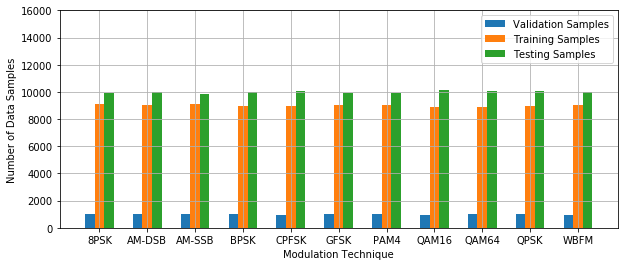
\includegraphics[scale=0.6]{stratSampleModTech}
	\caption{Histogram of Partitioned Data, grouped by Modulation Technique}
	\label{strat-sample}
%	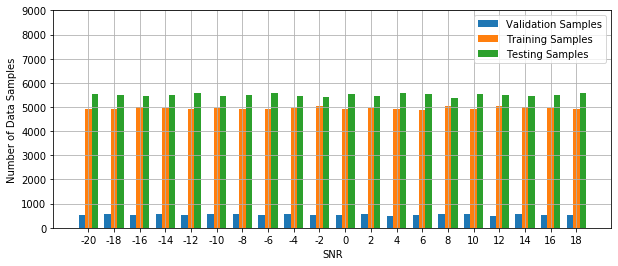
\includegraphics[scale=0.6]{stratSampleSNR}
%	\caption{Histogram of Partitioned Data, grouped by SNR}		
\end{figure}

The Keras framework is able to reserve a portion of the training set for validation purposes at the time of training. However, the source of entropy for this is not within the user's control. Data was manually partitioned (using seeded pseudo-random number generators) in an effort to ensure that datasets stayed the same across different tests.

\section{Artificial/Deep Neural Network (A/DNN) Solution}

\subsection{Background}

Artificial Neural Networks (ANNs) are models inspired by biological neurons. Artificial neurons can get "activated" by certain inputs and an arrangement of such neurons connected together using weighted links can be used for classification or regression tasks. These networks can be trained by updating connection weights via feedback from outputs. The earliest neural networks only had a single layer which connected the input and output layers. Deep Neural Networks (DNNs) are ANNs with multiple layers in between the input and output layers. DNNs have proved to be useful in dealing with complicated problems that conventional ANNs could not otherwise solve. These days, the term DNN and ANN both refer to fully connected feed forward neural networks and in the context of this work they mean one and the same. These two terms may be used interchangeably but they refer to the same thing unless stated otherwise.

\subsection{Related Work}

DNNs are ubiquitous in regression and classification tasks. For the AMC task, certain features can provide sufficient separation between modulation classes. The most commonly used features are cumulants. Cumulants are statistical quantities determined using the moments of a probability distribution. Identical distributions will tend to, ideally, have identical cumulants. In \cite{ann1}, Lee \textit{et al} conducted an analysis of several second-order, fourth-order and sixth-order cumulants in order to determine which combination of these cumulants would help with AMC for five modulation schemes. They demonstrate that $C_{20}$, $C_{41}$, $C_{42}$ and $C_{63}$ can help discriminate between PSK and QAM modulation schemes. These cumulants are some of the features that have been used in my DNN.

Narendar \textit{et al} \cite{c42norm} suggest the use of a normalized version of the fourth order cumulant, $C_{42}$, such that $C^N_{42}=\frac{C_{42}}{\left(C_{21}\right)^2}$. They are able to use this normalized $C_{42}$ to achieve good classification results in their AMC system. It should be noted that while their approach to AMC does not make use of neural networks, it is still based on pattern recognition. Neural networks are all about identifying patterns and so, their idea will no doubt be useful in this project.

In \cite{ann2}, Kim \textit{et al} propose a DNN based solution to AMC that makes use of 21 features extracted from the input signal. Unfortunately, their rationale behind choosing these features isn't clear. Most of these 21 features are based on distribution-based statistics and are either cumulants or other quantities derived from moments (Kurtosis and Skewness). The remaining features are derived from statistics related to characteristics of the input signal such as instantaneous amplitude, phase and power. I found 7 of these features: $C_{40}$, $C_{63}$, $C_{80}$, Kurtosis, Skewness, Peak-to-Rms Power Ratio and Peak-to-average Power Ratios to be useful and have made use of the same in my DNN implementation.

\subsection{Feature Vector}

The input to the DNN is a vector that made up of eleven features that are extracted from the input signal. These features have been selected based on their popularity in the AMC domain as well as for their ability to discriminate between the different modulation classes. These eleven features are defined below.

Let $a=a_I[n]+ja_Q[n]$ be an input signal, whose samples contain the in-phase and quadrature phase components, represented in rectangular notation.

Let $E[.]$ denote the Expectation operator

Let $M_{x,y}=E[(r[n])^{x-y}(r^*[n])^y]$ denote the $(x+y)^{th}$ Order Moment of $r[n]$ 

\begin{enumerate}
\setlength{\itemsep}{1.2\baselineskip}
\item Cumulant, $\mid C_{20} \mid\ =\ \mid E\left[a^{2}\left(n\right)\right]\mid$
\item Cumulant, $\mid C_{21} \mid\ =\ \mid E\left[a\left(n\right)^{2}\right]\mid$
\item Cumulant, $\mid C_{40} \mid\ =\ \mid M_{40}-3M_{20}^2\mid$
\item Cumulant, $\mid C_{41} \mid\ =\ \mid M_{40}-3M_{20}M_{21}\mid$
\item Cumulant, $\mid C_{42}^Norm \mid\ =\ \mid \frac{M_{42}-M_{20}^2-2M_{21}^2}{C_{21}^2}\mid$
\item Cumulant, $\mid C_{63} \mid\ =\ \mid M_{63}-9M_{21}M_{42}+12M_{21}^3-3M_{20}M_{42}-3M_{22}M_{41}+18M_{20}M_{21}M_{22} \mid$
\item Cumulant, $\mid C_{80} \mid\ =\ \mid M_{80}-35M_{40}^2-28M_{60}M_{20}+420M_{40}-630M_{20} \mid$
\item Kurtosis, $K=\ \mid\frac{E\left[a-E\left[a\right]\right]^4}{E\left[\left(a-E\left[a\right]\right)^2\right]^{2}}\mid$ 
\item Skewness, $S=\ \mid\frac{E\left[a-E\left[a\right]\right]^3}{E\left[\left(a-E\left[a\right]\right)^2\right]^{\frac{3}{2}}}\mid$
\item Peak-to-RMS Power Ratio, $PR = \frac{max\left(\mid a \mid^2\right)}{\frac{1}{N}\sum_{i=1}^{N}\left(a[i]\right)^2}$
\item Peak-to-average Power Ratio, $PA = \frac{max\left(\mid a \mid\right)}{\frac{1}{N}\sum_{i=1}^{N}a[i]}$

\end{enumerate}

\subsection{Network Design}

A number of DNN architectures were constructed and trained. The performance of each was then evaluated based on their performance on the validation set. DNN-AV was the best performing network that had the lowest validation loss of \textbf{1.5647} (which occurred at the 70th Epoch). It also had the highest prediction accuracy of \textbf{43.02\%} (average across all modulation classes) on the validation set. The loss and accuracy curves for DNN-AV have been displayed in Figure \ref{fig:performanceDNN}. 

The architecture of DNN-AV has been detailed in TABLE \ref{tab:dnn-arch}. Other design specifics have been detailed in TABLE \ref{tab:dnnDesPar}. The initial design was a much simpler two-layer network which was grown in stages. Increasing the number of neurons and layers did increase performance somewhat but extending the network either in width or length beyond the final design of DNN-AV tended to yield diminishing returns as the performance gain was not justified when considering in the amount of parameters to be trained. Larger networks are prone to overfitting and Dropout regularization as well as early stopping helped ensure that the network would not just memorize the training data.

\begin{table}[]
\centering
\caption{Architecture of DNN-AV}
\label{tab:dnn-arch}
\begin{tabular}{lccc}
\hline
Layer & Layer Type & Description        & Activation \\ \hline
1     & Dense      & 4096 Units         & ReLU       \\
2     & Dropout    & Dropout Rate = 0.5 & -          \\
3     & Dense      & 2048 Units         & ReLu       \\
4     & Dropout    & Dropout Rate = 0.5 & -          \\
5     & Dense      & 1024 Units         & ReLu       \\
6     & Dropout    & Dropout Rate = 0.5 & -          \\
7     & Dense (Output)      & Units = 11         & SoftMax    \\ \hline
\end{tabular}
\end{table}

\begin{table}[]
\centering
\caption{Other Design Choices}
\label{tab:dnnDesPar}
\begin{tabular}{@{}ll@{}}
\toprule
Parameter                          & Description                               \\ \midrule
Loss Function                      & Categorical Cross-Entropy                 \\
Weight Optimizer                   & Adam                                      \\
Activation Function (Hidden Layer) & ReLU                                      \\
Activation Function (Output Layer) & SoftMax                                   \\
Regularization                     & Dropout, Early Stopping                   \\
Weight Initialization              & Xavier Initialization ('Glorot\_Uniform') \\
Batch Size                         & 1024                                      \\ \bottomrule
\end{tabular}
\end{table}

\begin{figure*}[h]
    \centering
    \begin{subfigure}[b]{0.4\textwidth}
        \centering
        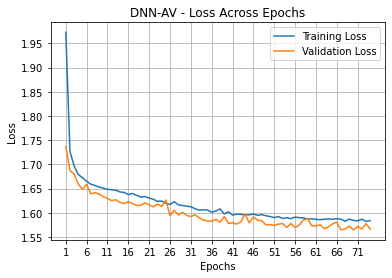
\includegraphics[scale=0.5]{dnnavPerf}
        \caption{Training Performance}
    \end{subfigure}%
    ~ 
    \begin{subfigure}[b]{0.4\textwidth}
        \centering
        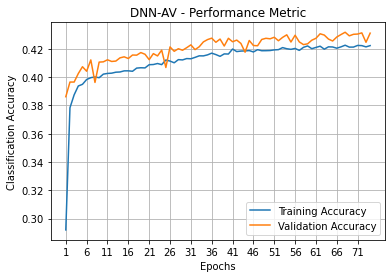
\includegraphics[scale=0.5]{dnnavPerfMet}
        \caption{Performance Metric}
    \end{subfigure}
    \caption{DNN-AV - Accuracy and Loss During Training}
    \label{fig:performanceDNN}
\end{figure*}

\subsection{Observations}


\begin{figure*}[h]
    \centering
    \begin{subfigure}[b]{0.5\textwidth}
        \centering
        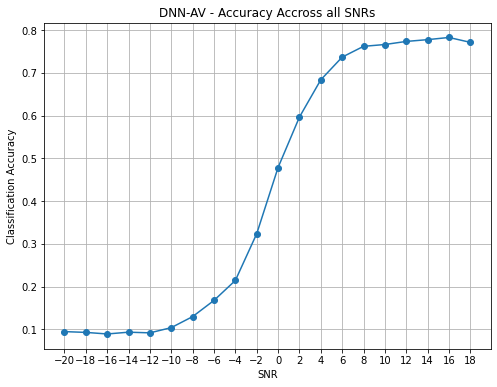
\includegraphics[scale=0.5]{dnnACCSNR}
        \caption{Performance Metric}
        \label{dnnACCSNR}
    \end{subfigure}%
    ~ 
    \begin{subfigure}[b]{0.5\textwidth}
        \centering
        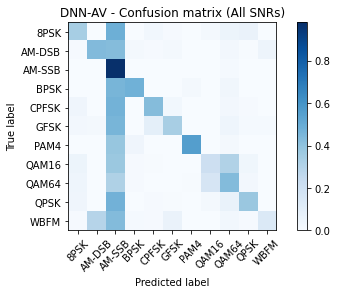
\includegraphics[scale=0.7]{dnnoverallConfMat}
        \caption{Confusion Matrix}
        \label{dnnConfMat}
    \end{subfigure}
    \caption{Performance of DNN-AV on Test Data}
\end{figure*}

\begin{figure}[!ht]
   \centering
   \subfloat[][]{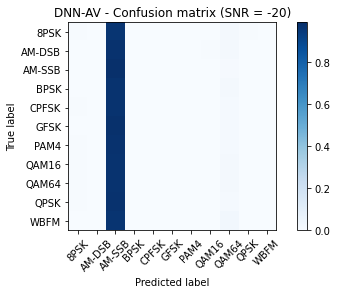
\includegraphics[width=.4\textwidth]{-20dnn}}\quad
   \subfloat[][]{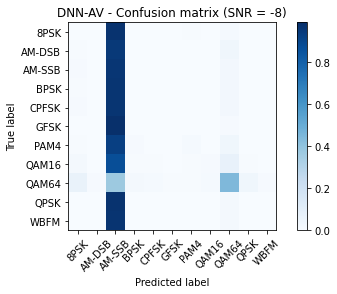
\includegraphics[width=.4\textwidth]{-8dnn}}\\
   \subfloat[][]{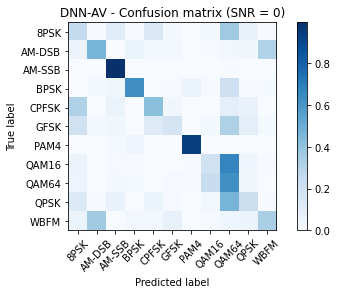
\includegraphics[width=.4\textwidth]{0dnn}}\quad
   \subfloat[][]{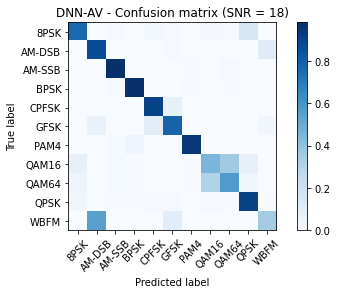
\includegraphics[width=.4\textwidth]{18dnn}}
   \caption{DNN-AV Confusion Matrices at Different SNRs}
   \label{fig:dnnConfSep}
\end{figure}

Figure \ref{dnnACCSNR} displayes the average classification accuracy (across all modulation classes) that DNN-AV achieves at each SNR level. The corresponding confusion matrix is shown in Figure \ref{dnnConfMat}. Figure \ref{fig:dnnConfSep} shows confusion matrices at different SNR values. There's not a lot of difference between the confusion matrices at -20 dB and -8 dB. The DNN does not perform well for input signals having a low SNR. This isn't all that surprising since the features extracted from a noisy signal will no doubt be contaminated. Observing the confusion matrix at 0 dB, we can start to see the main diagonal form. At this stage, AM-SSB and PAM-4 have relatively high classification accuracies. Note how the DNN is unable to distinguish between QAM-16 and QAM-64. At higher SNRs (greater than 4 dB, Figure \ref{dnnACCSNR}), the DNN starts performing much better. At 18 dB we can observe a nearly clean diagonal. Pay attention to the confusion matrix and you can see that there is some distinctions between the QAM-16 and QAM-64 classes.

\section{Convolutional Neural Network (CNN) Solution}

\subsection{Background}

CNNs take inspiration from the mammalian visual system. In particular, the way how the brain processes visual information hierarchically often starting with simple structures such as oriented edges \cite{catEye}. In the late 70s, Fukushima applied this idea to create the Neocognitron \cite{neocognitron}, a predecessor to CNNs, which was built to detect handwritten characters. The Neocognitron introduced the notion of a convolutional layer which was a spatially invariant filter that could be used to detect features irrespective of location in an image. The coefficients of the convolutional filter still had to be trained via some supervised learning algorithm. Fast forward to 1998, when LeCun \textit{et al} \cite{lenet5} applied error backpropagation to train convolutional filter coefficients pavinf the way to CNNs as we now know them.

While CNNs, like UNet \cite{unet} may be built using convolutional layers alone, they often make use of fully connected neurons when performing classification. In a CNN designed for classification, the convolutional layers essentially perform feature extraction in a hierarchical manner starting with low-level features in the first convolutional layer.

\subsection{Related Work}

CNNs are commonly used in problems where the input data consist of images. However, they can be useful in any task where data has features that are spatially relevant such as in the case of text classification or speech recognition. Along the same lines, CNNs can be useful in AMC where the input data is made up of a combination of a finite number of symbols that are unique for a given modulation scheme. 

There are a lot of papers that present the solutions to the AMC problem. Each paper proposes one type of network design or the other and claims it to be best suited to the task. However, there’s often nothing more than empirical evidence to back these claims. This sort of situation is also commonplace in other domains, such as computer vision for instance, where neural networks are rampant.

That said, a number of recent publications were reviewed in an effort to identify “best-practices” that have proven helpful for designing a CNN for AMC. O’Shea \textit{et al} \cite{cnn2} achieve reasonably good performance on the RADIOML 2016.10A dataset with two CNN based networks. These networks are able to get over 10\% accuracy for the lowest SNRs and above 80\% accuracy for higher SNRs. Both networks consist of two convolutional layers and a fully connected layer (excluding the final classification layer). They differ only in that one design has more filters in the convolutional layers that the other. Both networks make use of the Adam optimizer as well as dropout for regularization. A lot of details are left to interpretation. Ramjee \textit{et al} \cite{cnn1} make use of a deeper CNN design with four convolutional layers based on the more complex CNN proposed in \cite{cnn2}. While they report a higher accuracy at high SNRs (over 80\% at 18dB), their network does not do well at the lower SNRs. 

Lee and colleagues propose an interesting solution in \cite{featImage} wherein they first extract a number of statistical features (such as higher order cumulants) which are then used to compose a “feature image” that is then fed into a CNN. Their claim is that feature images are distinct for a given modulation technique. The results they report indicate an improvement in the accuracies at high SNRs (nearly 100\% over 4dB). The performance at lower SNRs were not very remarkable.

In \cite{ddriven}, Wang and Yang highlight a problem that I have observed during my experiments. It is difficult for most CNNs that operate on the input signal in rectangular form to differentiate between QAM-16 and QAM-64 modulation even at the highest SNR. The authors use an additional CNN used exclusively to differentiate between QAM-16 and QAM-64. This secondary network uses constellation diagrams as input.

\subsection{Network Design} 

\begin{table}
\centering
\caption{Architecture of CNN-AV}
\label{tab:my-table-1a}
\begin{tabular}{@{}cccc@{}}
\toprule
Layer & Layer Type  & Description                               & Activation \\ \midrule
1     & Convolution & 512 Filters, Size = (1,3), Stride = (1,1) & ReLU       \\
2     & MaxPooling  & Window = (1,2), Stride = (1,2)            & -          \\
3     & Dropout     & Dropout Rate = 0.5                        & -          \\
4     & Convolution & 256 Filters, Size = (1,3), Stride = (1,1) & ReLu       \\
5     & MaxPooling  & Window = (1,2), Stride = (1,2)            & -          \\
6     & Dropout     & Dropout Rate = 0.5                        & -          \\
7     & Convolution & 128 Filters, Size = (1,3), Stride = (1,1) & ReLu       \\
8     & MaxPooling  & Window = (1,2), Stride = (1,2)            & -          \\
9     & Dropout     & Dropout Rate = 0.5                        & -          \\
10    & Convolution & 64 Filters, Size = (1,3), Stride = (1,1)  & ReLu       \\
11    & MaxPooling  & Window = (1,2), Stride = (1,2)            & -          \\
12    & Dropout     & Dropout Rate = 0.5                        & -          \\
13    & Dense       & Units = 128                               & ReLu       \\
14    & Dense (Output)       & Units = 11                                & SoftMax    \\ \bottomrule
\end{tabular}%
\end{table}

Several CNN designs were constructed and trained using the same training set. These designs were then compared based their performances on the same validation set. CNN-AV was the best performing network with the lowest validation loss of \textbf{1.2095} (which occurred at the 46th Epoch). It also achieved the highest Average Classification Accuracy (across all modulation techniques) of \textbf{53.81\%} on the validation set. The loss and accuracies across the number of training Epochs have been displayed in Figure \ref{fig:performanceCNN}. The architecture of CNN-AV has been detailed in TABLE \ref{tab:my-table-1a}. Other design choices for CNN-AV have been detailed in TABLE \ref{tab:my-table-1b}.

Like in the case of the DNN, the design process for the CNN based network was highly empirical. The existence of Pooling layers significantly increased the number of hyper parameters that could be tuned. While the final design for CNN-AV is large, training was still manageable on account of these pooling layers. They helped reduce the dimensionality of outputs coming out of a layer meaning lesser connections and trainable weights to subsequent layers. 

% Please add the following required packages to your document preamble:
% \usepackage{booktabs}
\begin{table}[]
\centering
\caption{Other Design Choices}
\label{tab:my-table-1b}
\begin{tabular}{@{}ll@{}}
\toprule
Parameter                          & Description                               \\ \midrule
Loss Function                      & Categorical Cross-Entropy                 \\
Weight Optimizer                   & Adam                                      \\
Activation Function (Hidden Layer) & ReLU                                      \\
Activation Function (Output Layer) & SoftMax                                   \\
Regularization                     & Dropout, Early Stopping                   \\
Weight Initialization              & Xavier Initialization ('Glorot\_Uniform') \\
Batch Size                         & 1000                                      \\ \bottomrule
\end{tabular}
\end{table}

\begin{figure*}[h]
    \centering
    \begin{subfigure}[b]{0.4\textwidth}
        \centering
        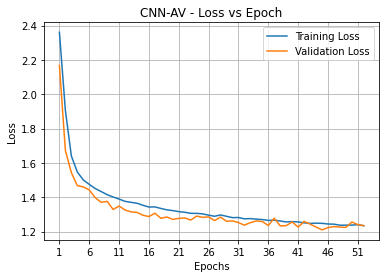
\includegraphics[scale=0.5]{cnnavPerf}
        \caption{Training Performance}
    \end{subfigure}%
    ~ 
    \begin{subfigure}[b]{0.4\textwidth}
        \centering
        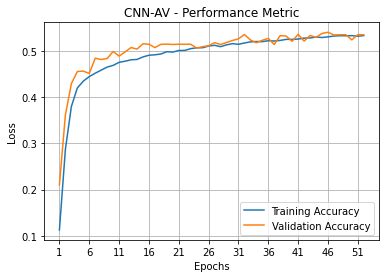
\includegraphics[scale=0.5]{cnnavPerfMet}
        \caption{Performance Metric}
    \end{subfigure}
    \caption{CNN-AV - Accuracy and Loss During Training}
    \label{fig:performanceCNN}
\end{figure*}

\subsection{Observations}

Figure \ref{cnnACCSNR} displays the average classification accuracy (across all modulation classes) that CNN-AV achieves at each SNR level. The corresponding confusion matrix is shown in Figure \ref{cnnConfMat}. Figure \ref{fig:cnnConfSep} shows confusion matrix plot for specific SNR values. At -20 dB, CNN-AV has poor performance with all inputs signals classified as AM-SSB. The performance gets better as SNR increases. At SNRs greater than 0 dB, the performance improvement is minimal as seen from Figure \ref{fig:cnnConfSep} (c) and (d). While there is a slight improvement, QAM-16 signals are still misclassified as QAM-64. These two modulation schemes are essentially the same and differ only by the number of bits used to encode symbols. It appears that the CNN is unable to discern between the two just based on the signal waveform.

\begin{figure*}[h]
    \centering
    \begin{subfigure}[b]{0.5\textwidth}
        \centering
        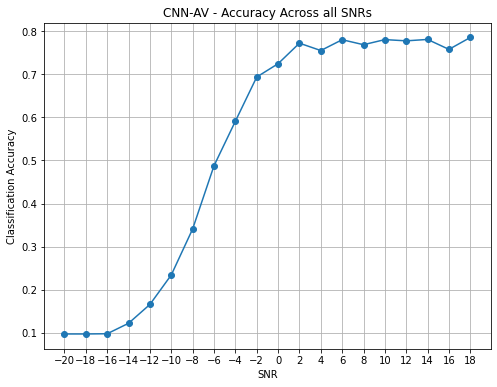
\includegraphics[scale=0.5]{cnnACCSNR}
        \caption{Performance Metric}
        \label{cnnACCSNR}
    \end{subfigure}%
    ~ 
    \begin{subfigure}[b]{0.5\textwidth}
        \centering
        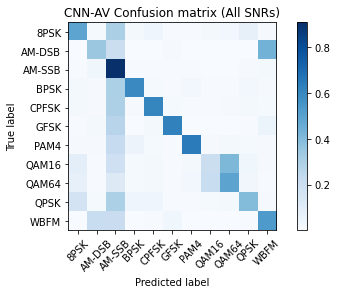
\includegraphics[scale=0.7]{cnnoverallConfMat}
        \caption{Confusion Matrix}
    \end{subfigure}
    \caption{Performance of CNN-AV on Test Data}
    \label{cnnConfMat}
\end{figure*}

\begin{figure}[!ht]
   \centering
   \subfloat[][]{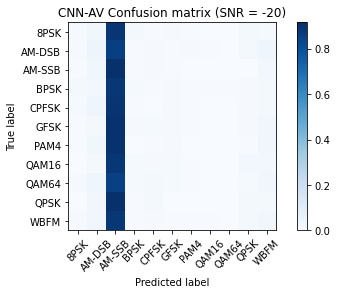
\includegraphics[width=.4\textwidth]{-20}}\quad
   \subfloat[][]{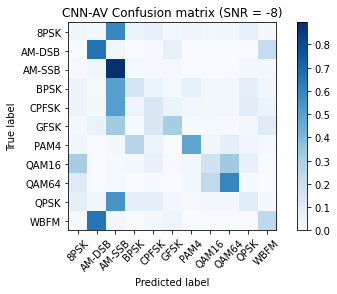
\includegraphics[width=.4\textwidth]{-8}}\\
   \subfloat[][]{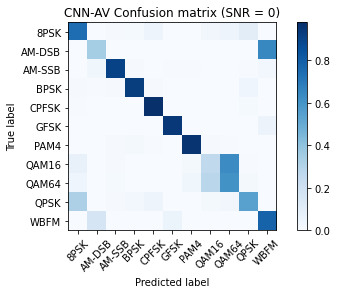
\includegraphics[width=.4\textwidth]{0}}\quad
   \subfloat[][]{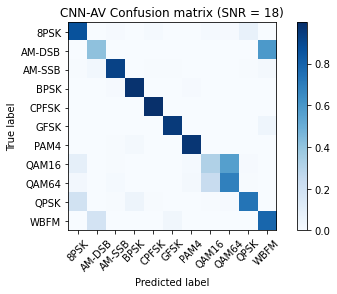
\includegraphics[width=.4\textwidth]{18}}
   \caption{CNN-AV Confusion Matrices at Different SNRs}
   \label{fig:cnnConfSep}
\end{figure}

\section{Discussion}

The average prediction accuracy across modulation classes has been the performance metric used in this project. The performance metric across the training, testing and validation sets have been reported in the TABLE \ref{tab:discuss}. Both networks perform nearly identically when the input signal has a high SNR. For inputs signals at lower SNR levels, the CNN based architecture performs relatively better as it is able to reasonably distinguish between modulation classes at SNR values as low as -4 dB (around 60\% accuracy). The difference in performance at low SNRs is most likely due to the nature of how each architecture fundamentally functions.

\begin{table}[h]
\centering
\caption{Average Prediction Accuracy Across All Modulation Classes (Performance Metric)}
\label{tab:discuss}
\begin{tabular}{ccc}
\hline
\multirow{2}{*}{} & \multicolumn{2}{c}{Network} \\
                  & DNN-AV       & CNN-AV      \\ \hline
Training Set      & 42.12\%      & 52.93\%     \\
Validation Set    & 43.02\%      & 53.81\%     \\
Test Set          & 42.64\%      & 53.04\%     \\ \hline
\end{tabular}
\end{table}

The CNN processes the input signal by looking at signal amplitudes. This is more or less equivalent to observing the signal waveform. Convolutional layers are then trained such that they activate when specific features are identified. It does seem then that even at lower SNRs the CNN is still able to discern some of these features unique to different modulation classes.

In case of the DNN, feature extraction is a separate process and the network sees only what it is fed as input. Unfortunately, the onus is on the designer to ensure that the right features are passed to the network. Without a sufficient understanding of the problem, incorrect features fed into the network will not help the network to learn. It does seem then that the features I chose as input to DNN-AV were easily affected by noise. Perhaps identifying and extracting other features which are more resilient to noise can help improve the performance at lower SNRs.

Another point of note relates to the ambiguity between QAM-16 and QAM-64. While CNN-AV could not make the distinction even at the highest SNR levels, DNN-AV performed somewhat better at 18 dB (refer to Figure \ref{fig:dnnConfSep} (d)).

\section{Conclusion}

In conclusion, both DNNs and CNNs are viable approaches when attempting to tackle the task of Automatic Modulation Classification. While CNNs are great at extracting features from input, they come at a cost of increased computation. DNNs on the other hand are much simpler but are only efficient if they're given the right kind of feature inputs.

% use section* for acknowledgment
%\section*{Acknowledgment}

% Can use something like this to put references on a page
% by themselves when using endfloat and the captionsoff option.
\ifCLASSOPTIONcaptionsoff
  \newpage
\fi



% trigger a \newpage just before the given reference
% number - used to balance the columns on the last page
% adjust value as needed - may need to be readjusted if
% the document is modified later
%\IEEEtriggeratref{8}
% The "triggered" command can be changed if desired:
%\IEEEtriggercmd{\enlargethispage{-5in}}

% references section

% can use a bibliography generated by BibTeX as a .bbl file
% BibTeX documentation can be easily obtained at:
% http://mirror.ctan.org/biblio/bibtex/contrib/doc/
% The IEEEtran BibTeX style support page is at:
% http://www.michaelshell.org/tex/ieeetran/bibtex/
%\bibliographystyle{IEEEtran}
% argument is your BibTeX string definitions and bibliography database(s)
%\bibliography{IEEEabrv,../bib/paper}
%
% <OR> manually copy in the resultant .bbl file
% set second argument of \begin to the number of references
% (used to reserve space for the reference number labels box)
\bibliographystyle{IEEEtran}
\bibliography{eece571MProjectReferences}

% biography section
% 
% If you have an EPS/PDF photo (graphicx package needed) extra braces are
% needed around the contents of the optional argument to biography to prevent
% the LaTeX parser from getting confused when it sees the complicated
% \includegraphics command within an optional argument. (You could create
% your own custom macro containing the \includegraphics command to make things
% simpler here.)
%\begin{IEEEbiography}[{\includegraphics[width=1in,height=1.25in,clip,keepaspectratio]{mshell}}]{Michael Shell}
% or if you just want to reserve a space for a photo:

%\vfill

% Can be used to pull up biographies so that the bottom of the last one
% is flush with the other column.
%\enlargethispage{-5in}



% that's all folks
\end{document}


